\documentclass[12pt]{article}
\usepackage{latexsym}
\usepackage{fancyhdr}
\usepackage{amssymb,amsmath,amsthm}
\usepackage[pdftex]{graphicx}
\usepackage{pdfpages}
\usepackage[margin=1in]{geometry}


% Create answer counter to keep track of seperate responses
\newcounter{AnswerCounter}
\newcounter{SubAnswerCounter}
\setcounter{AnswerCounter}{1}
\setcounter{SubAnswerCounter}{1}

% Create answer environment which uses counter
\newenvironment{answer}[0]{
  \setcounter{SubAnswerCounter}{1}
  \bigskip
  \textbf{Solution \arabic{AnswerCounter}}
  \\
  \begin{small}
}{
  \end{small}
  \stepcounter{AnswerCounter}
}

\newenvironment{subanswer}[0]{
  (\alph{SubAnswerCounter})
}{
 \bigskip
  \stepcounter{SubAnswerCounter}
}

% Allows easy use of vectors
\newcommand{\vect}[1]{\vec{\boldsymbol{#1}}}

% Setting up the title
\title{Mathematics 131 \\
Topology I}
\author{
        Luis Antonio Perez \\
        HUID: 70871564 \\
        Harvard College \\
        \href{mailto:luisperez@college.harvard.edu}{luisperez@college}
}
\date{\today}

% Custom Header information on each page
\pagestyle{fancy}
\lhead{HUID: 70871564}
\rhead{Perez - \thepage}
\renewcommand{\headrulewidth}{0.1pt}
\renewcommand{\footrulewidth}{0.1pt}

% Title page is page 0
\setcounter{page}{0}

\begin{document}
\begin{answer}
We now present the outline for the proof of the lifting lemma. First, we make a statement of the theorem and make sure what it says is understood.
\begin{proof}[The General Lifting Lemma]
Let $p: E \to B$ be a covering map, let $p(e_0) = b_0$. Let $f: Y \to B$ be a continuous map, with $f(y_0) = b_0$. Suppose $Y$ is path connected and locally path connected. The map $f$ can be lifted to a map $\tilde{f} : Y \to E$ such that $\tilde{f}(y_0) = e_0$ if and only if
$$
f_*(\pi_1(Y,y_0)) \subset p_*(\pi_1(E,e_0))
$$
Furthermore, if the lifting exists, then it is unique.
\end{proof}
Let us make sure we understand the theorem.
\begin{itemize}
\item As always, we have a space $B$ and a layer of pancakes $E$ which is the covering space. Normally, with the standard lifting lemma, we can lift paths on $B$ to paths on $E$.
\item With this more general lifting lemma, we can actually take any continuous map which traces out a path on $B$ (ie, take any $f: Y \to B$) with starting point $f(y_0) = b_0 \in B$.
\item There are some restrictions, in particular, $Y$ must be path connected and locally path connected.
\item The lemma states that the lifting is possible (and unique) only in the case where the image of the homomorphism induced by $f$ is a subset of the image of the homomorphism induced by $p$. Intuitively, it means that the equivalence classes of loops in $B$ under $f_*$ must be a subset of those in $B$ under $p_*$. Even more intuitively, it means that loops from $Y$ based at $y_0$ are taken to loops in $B$ based at $b_0$ when the corresponding loop in $E$ based at $e_0$ is also taken to $B$ based at $b_0$.
\end{itemize}

We now focus on first proving the second part of the if and only if. That is, that if the lifting $\tilde{f}$ exists, then
$$
f_*(\pi_1(Y,y_0)) = p_*(\tilde{f}_*(\pi_1(Y,y_0))) \subset p_*(\pi_1(E,e_0))
$$

To see the above:
\begin{itemize}
\item Let us consider the image of the homomorphic extension of $f$. As in put we take the equivalence classes of $\pi_1(Y,y_0)$, which are essentially loops in $Y$ based at $y_0$.
\item The extension $f_*$ maps these loops to loops based to $b_0$ in $B$.
\item Given that the lifting exists, we can actually first lift the paths from $Y$ onto $E$ using the homomorphic extension of the lifting. The loops are now loops in $E$ based at $e_0$, or a subset therefore. Then, we can project these paths back down onto $B$. This is exactly the image of $f_*$, where we now have a set of loops which are based at $b_0$, which can only be a subset of all loops one can project onto $B$ based at $e_0 \in E$\end{itemize}

The above clarifies the equations we wrote, thereby showing part of the theorem. We just need to argue that the lifting is unique.
\begin{itemize}
\item The lifting $\tilde{f}$ is unique. This is because path lifting are unique.
\item More clearly, take a path $\alpha$ in $Y$ from $y_0 \to y_1$ for some $y_1 \in Y$. Then consider the path $f \circ \alpha $ in $B$ and lift it to a unique path $\gamma$ in $E$ beginning at $e_0$.
\item Note, however, that $\tilde{f} \circ \alpha$ is lifting of $f \circ a$, and therefore we must have that $\tilde{f}(y_1) = \gamma(1)$, the endpoint of $\gamma$ because they both start at $e_0$.
\end{itemize}
The above shows the fact that if $\tilde{f}$ exists, the the image of its extension is a subset of the image of the homomorphic extension of the covering map. Furthermore, it is unique. \\

Next, we want to show the ``if'' part of the prove. This is to say, if:
$$
f_*(\pi_1(Y,y_0)) \subset p_*(\pi_1(E,e_0))
$$
then the lifting exists.

First, let us consider the lifting $\tilde{f}$. How do we construct this lifting, and how do we show that it is well-defined and continuous (a requirement for liftings). Well, it turns out that the intuition is relatively straightforward.
\begin{itemize}
\item Let us first choose a path $y_0 \to y_1$ for some $y_1 \in Y$, call it $\alpha.$
\item Then we can take this path $f \circ \alpha \in B$ and lift it to a path $y \in E$ beginning at $e_0$ using $p^{-1}$.
\item Next, we define $\tilde{f}(y_0) = e_0$ and $\tilde{f}(y_1) = \gamma(1)$.
\end{itemize}
The construction above works, as we now show. Fist, we focus on proving that the construction of $\tilde{f}$ is well-defined.
\begin{itemize}
\item We show that lifting two distinct paths with the same endpoints in $Y$ gives you two paths with the same endpoints in $E$.
\item Take two paths $\alpha$ and $\beta$ in $Y$ from $y_0 \to y_1$.
\item Lift the path in $B$ defined by $f \circ \alpha$ to $\gamma$, and then lift the path defined by $f \circ \bar{\beta}$ (this is the path going in the reverse direction from $f(y_1) \to f(y_0)$) to a path $\delta$. Then note that $\gamma * \delta$ is a lifting of the loop $f \circ (\alpha * \bar{\beta})$. By our assumption above, it must be the case that the equivalence class of this loop belongs to the image of $p_*$. Therefore, by Theorem 54.6, $\gamma * \delta$ is a loop in $E$. Therefore, note that $\bar{\delta}$ is a lifting of $f \circ \beta$, which is well-defined. \\
\end{itemize}

Now that we've shown that $\tilde{f}$ is well-defined, we just need to show that it is continuous.

\begin{itemize}
\item Let us focus first on proving the continuity of $\tilde{f}$ at the point $y_1 \in Y$. We prove continuity, we show that $\tilde{f}^{-1}$ maps open sets to open sets.
\item Take an open set $N$ in the image of $\tilde{f}$. That is, take an open set $N \subset E$ which contains the point $\tilde{f}(y_1)$.
\item To begin, we first choose a path connected neighborhood of $f(y_1) \in B$, call it $U$ which is evenly covered by $p$. We can do this by the definition of a covering map.
\item Look at the slices of $p^{-1}(U)$, and take $V$ to be the slice that contains $p^{-1}(f(y_0)) = p^{-1}(b_0) = \tilde{f}(y_0)$.
\item We can always choose the $U$ small enough so that $V \subset N$.
\item Then note that we can restrict $p \mid V : V \to U$, where $V$ is homeomorphic to $U$.
\item By continuity of $f$ and the path connectedness of $Y$, we can find a path-connected, open neighborhood $W$ of $y_1$ such that $f(W) \subset U$.
\item For $y \in W$, chose a path $\beta$ in $W$ from $y_1$ to $y$. Since $\tilde{f}$ is well defined, $\tilde{f}(y)$ can be obtained by taking the path $\alpha * \beta$ from $y_0 \to y$, and then lifting the path $f \circ (\alpha * \beta) $ to a path in $E$ beginning at $e_0$.
\item Note that $f(y)$ is the endpoint of this lifted path.
\item Note that the path $f \circ \beta$ lies completely in $U$, and therefore can take $p^{-1} \circ f \circ \beta$ as a lifting of this path onto $E$ that begins at $\tilde{f}(y_1)$.
\item Using the results from before, this means that $\gamma * \delta$ is a lifting of $f\circ (\alpha * \beta)$ that begins at $e_0$ (we're just concatenating paths).
\item The path ends at $\delta(1)$ of $V$.
\item Putting the above together, we have that $\tilde{f}(W) \subset V \subset N$ because every point $y \in W$ has a corresponding path fully contained in $V$.
\end{itemize}
The above shows that $\tilde{f}$ is well-defined and continuous, thereby proving the theorem.
\end{answer}

\begin{answer}
The covering spaces for the three-lobed graph are shown in Figure \ref{fig:covering_spaces}.

\begin{figure}[h!]
\centering
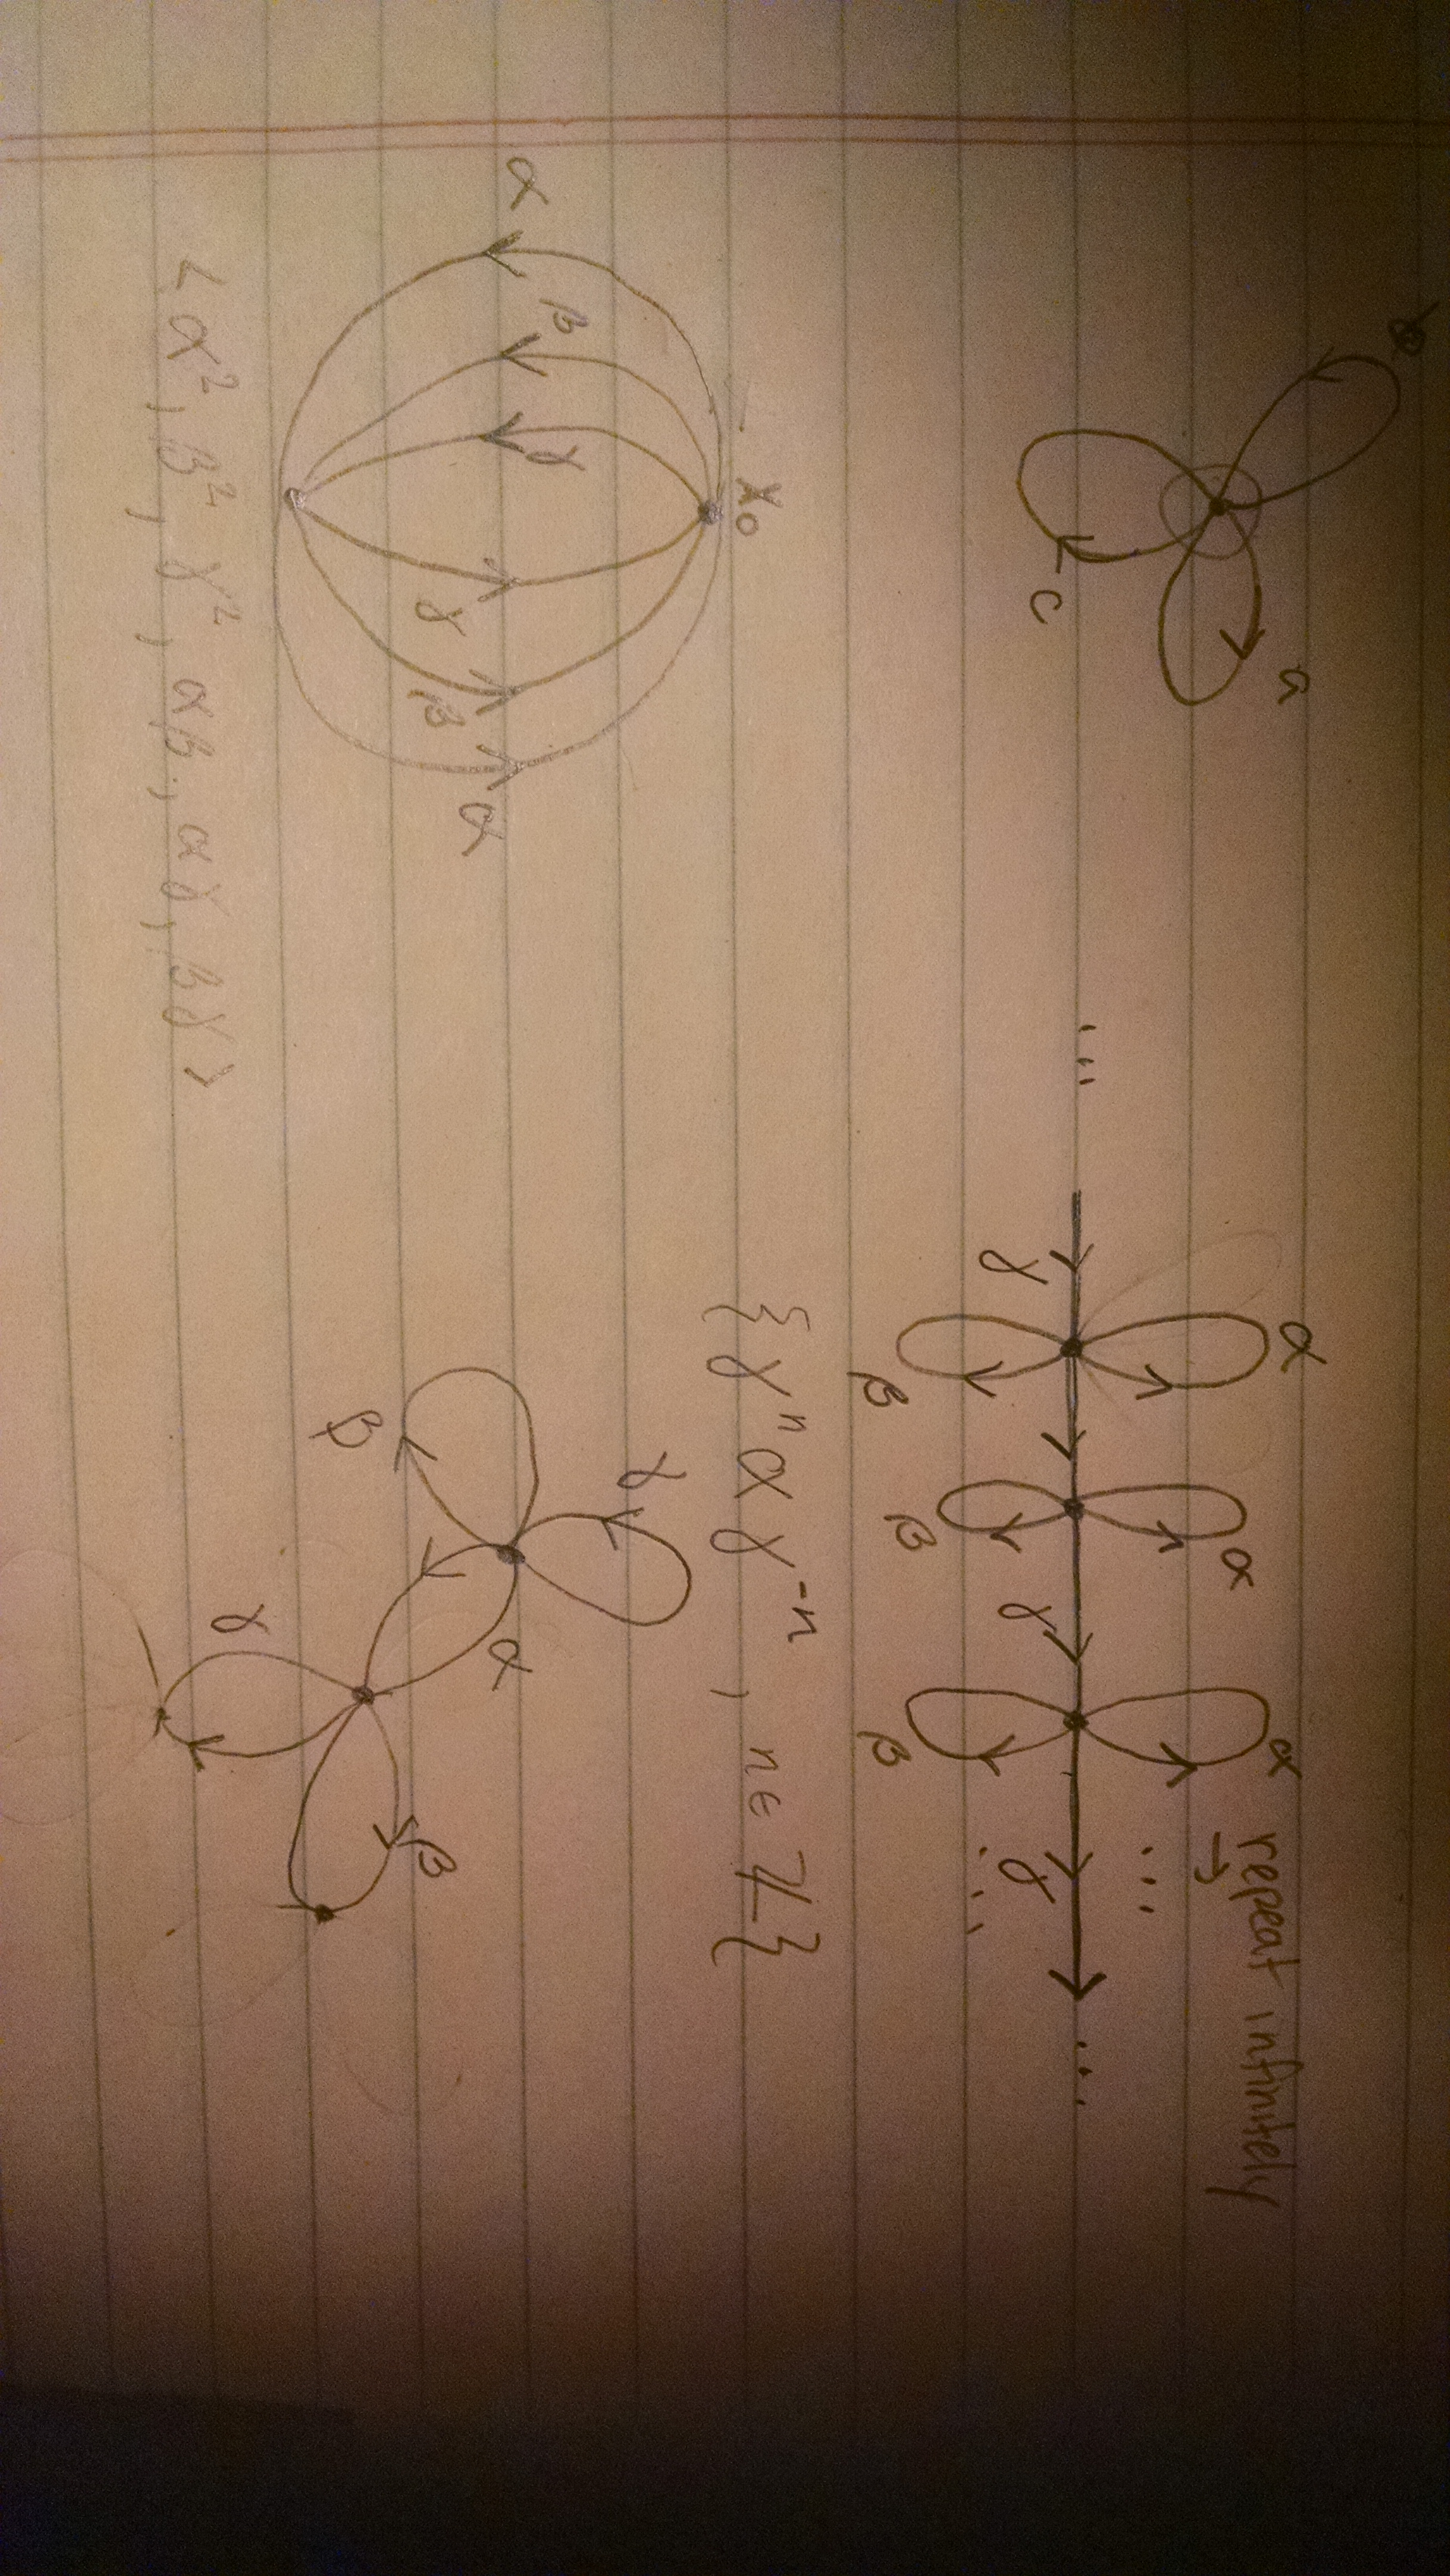
\includegraphics[scale=0.07,angle=90]{covering.jpg}
\caption{Non-trivial covering spaces of a three-lobed graph.}
\label{fig:covering_spaces}
\end{figure}
\end{answer}

\begin{answer}[Page 348, \#5]
We consider the covering map $p \times p: S^1 \times S^1$ of Example $4$ in Section 53. We also consider the path:
$$
f(t) = (\cos 2\pi t, \sin 2\pi t) \times (\cos 4\pi t, \sin 4\pi t)
$$
The sketch of this path can be seen in Figure \ref{fig:torus}.

\begin{figure}[h!]
\centering
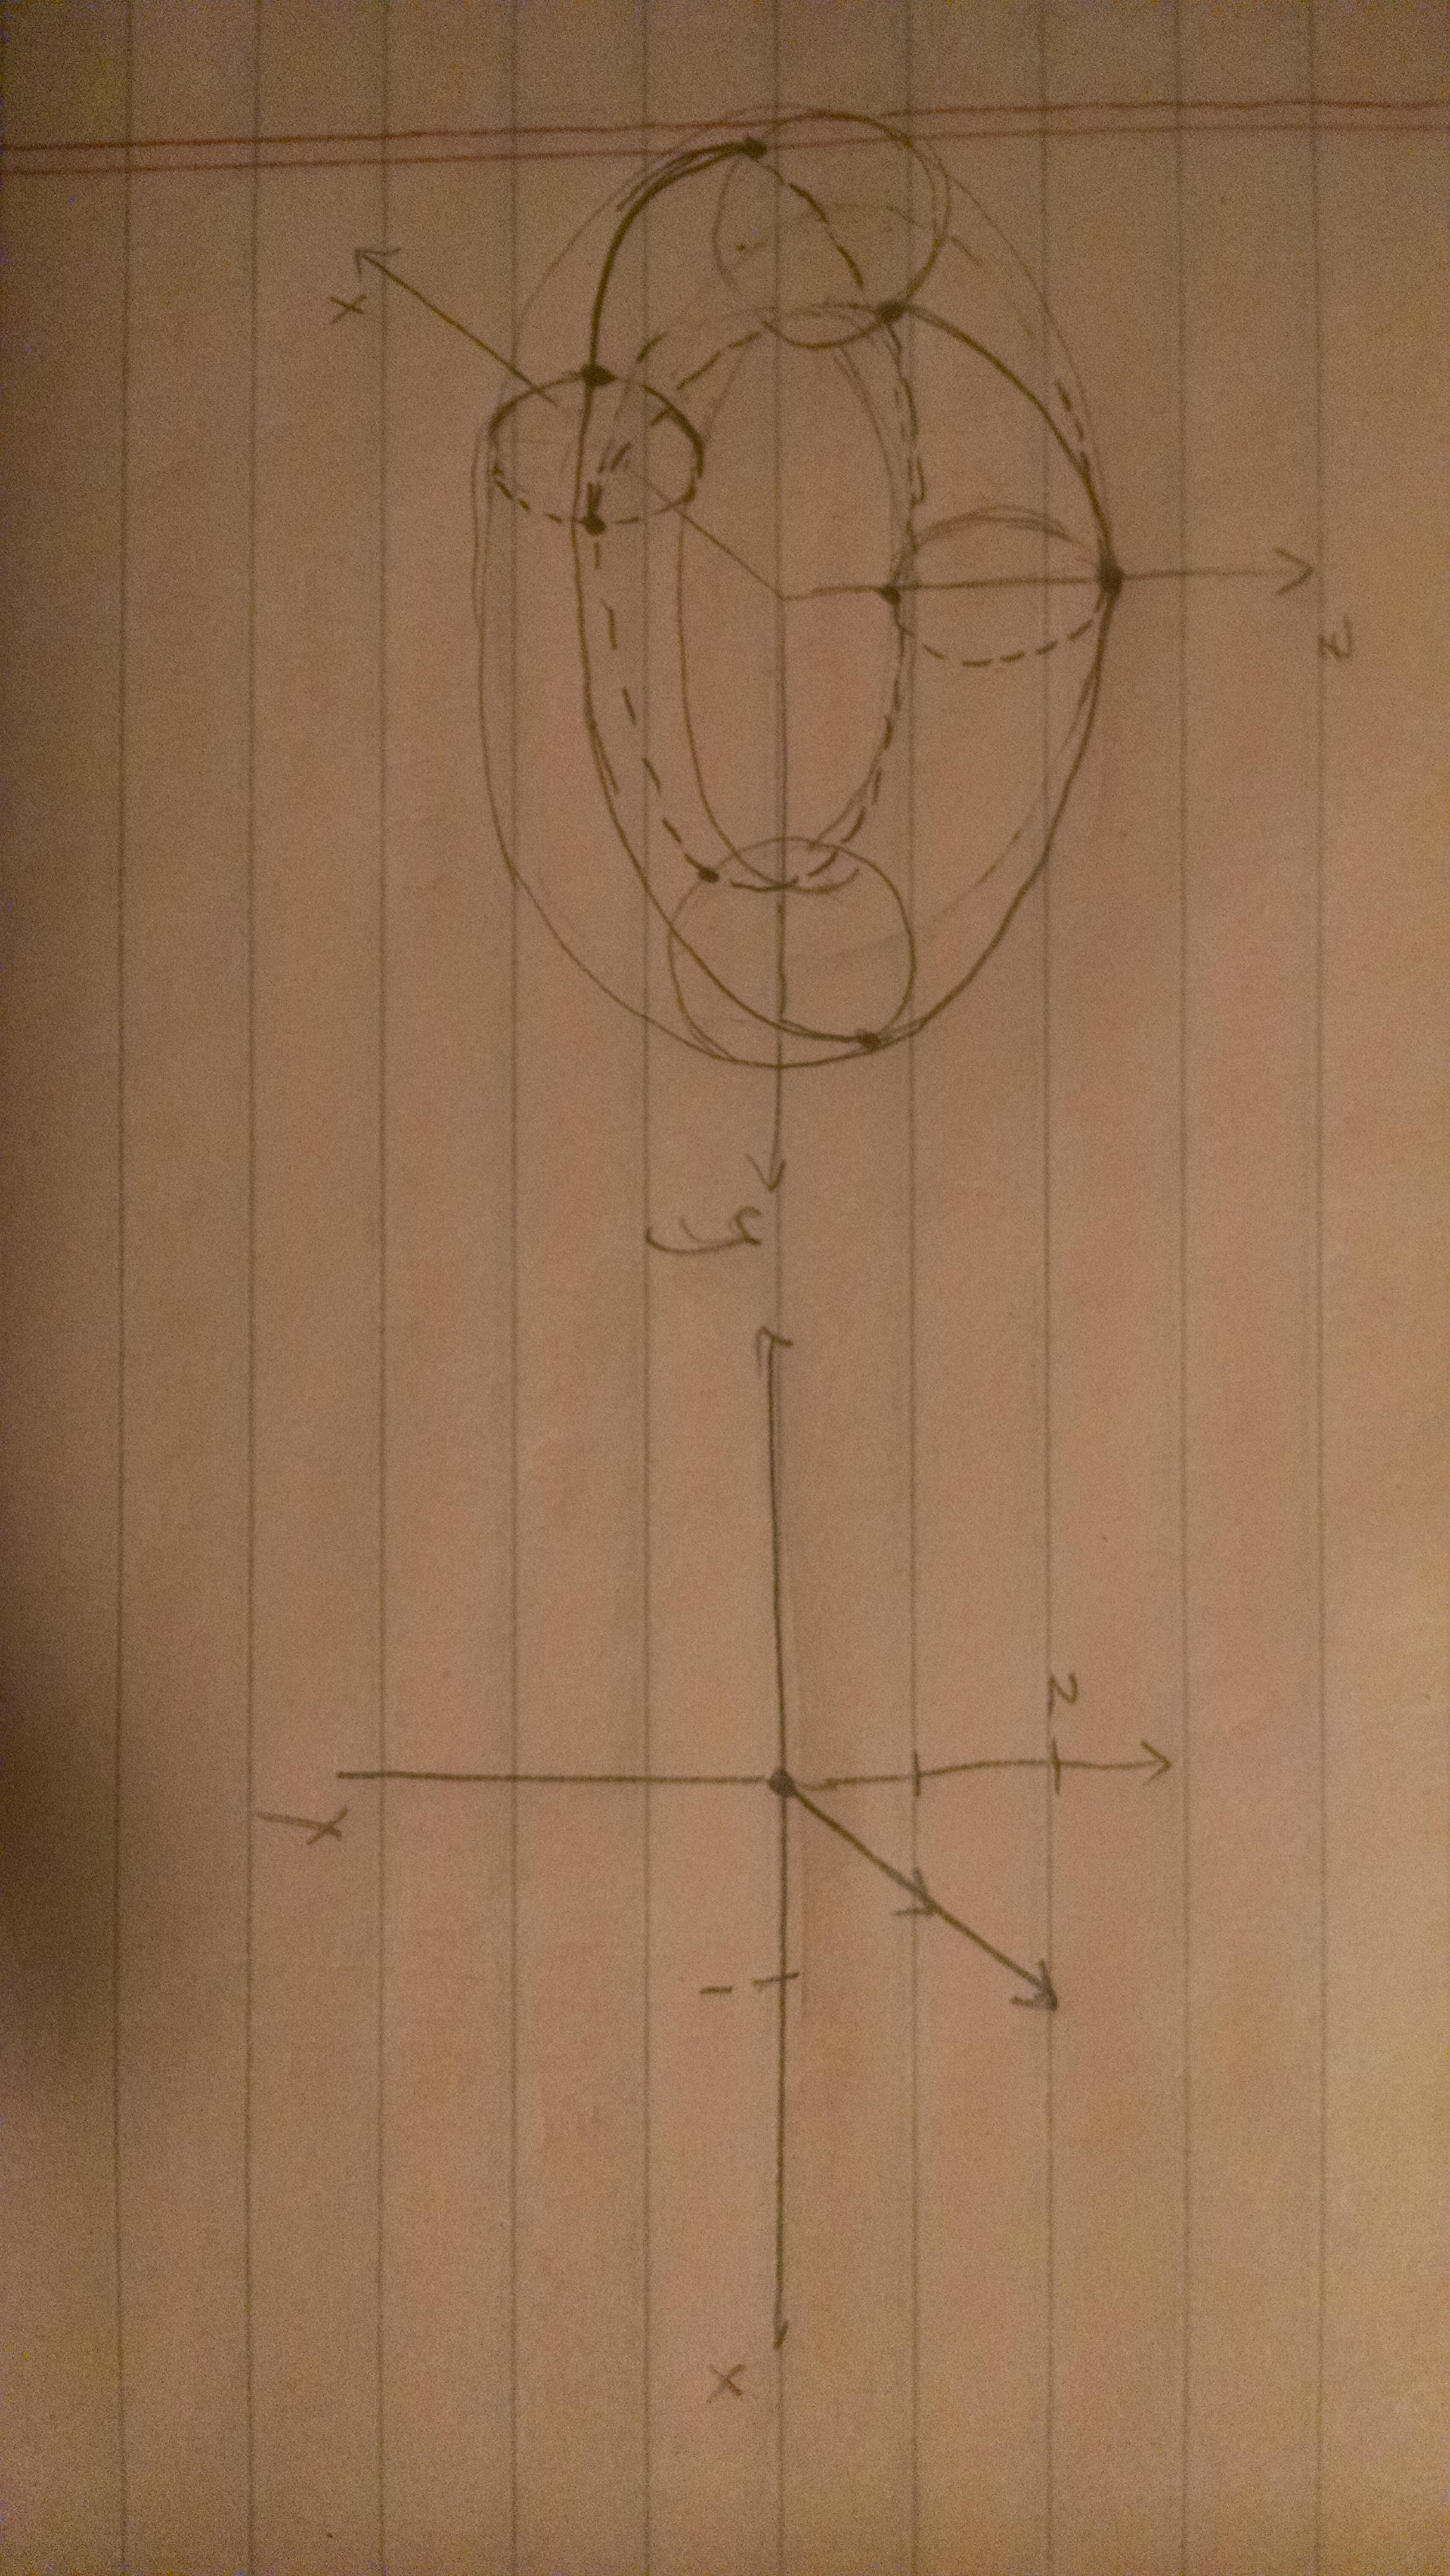
\includegraphics[scale=0.07, angle=90]{torus_lifting.jpg}
\caption{Sketch of a path on the Torus. The path essentially complete two complete cycles around the $z$-axis of the torus before completing one cycle of the circle on the $xz$-plane.}
\label{fig:torus}
\end{figure}

The lifting of $\tilde{f}: [0,1] \to \mathbb{R}^2$ is given by:
$$
\tilde{f}(t) = (t, 2t)
$$
for $t \in [0,1]$ beginning at $(0,0)$ and ending at $(1,2)$.

\end{answer}


\begin{answer}[Page 348, \#8]
We let $p: E \to B$ be a covering map, with $E$ path connected. We show that if $B$ is simply connected, then $p$ is a homeomorphism.
\begin{proof}
By definition of a covering, we know that $p: E \to B$ is a continuous surjective map. Therefore, all we need to show is that $p^{-1}: B \to E$ is also continuous. By Theorem 54.4, given that $E$ is path connected, we must have that:
$$
\phi: \pi_1(B,b_0) \to p^{-1}(b_0)
$$
is surjective. However, note that $| \pi_1(B,b_0)| = 1$ because $B$ is simply connected, therefore $|p^{-1}(b_0)| = 1$. Then by the connectedness of $B$, this implies that for all $b \in B$, $|p^{-1}(b)|= 1$. To see this, just note that we can start at the point $b_0$ which must have exactly $1$ element in the pre-image for some open neighborhood $U_{b_0}$. Note that for any $b \in U_{b_0}$, it must be the case that the same pre-image works. Therefore, by connectivity of $B$, for all $b \in B$, $|p^{-1}(b)| = 1$. Therefore, $p$ is a bijective convering map, and therefore a homeomorphism.
\end{proof}
\end{answer}


\begin{answer}[Page 483, \#1]
We show that if $n > 1$, then every continuous map $f: S^n \to S^n$  is nullhomotopic.
\begin{proof}
Note that $S^n$ for $n > 1$ is simply connected, so there exists a lift $\tilde{f}$ for every continuous map $f: S^n \to S^1$ such that $f = p \circ \tilde{f}$. Here, we lift $f$ to the universal cover. Note that the map $\tilde{f}$ is nulhomotopic by
$$
F(x,t) = (1-t)x
$$
Therefore, it must be the case that $f$ is also nulhomotopic, since homotopies lift.
\end{proof}
\end{answer}

\begin{answer}[Page 483, \#2]
We show two things:
\begin{enumerate}
\item Every continuous map $f: P^2 \to S^1$ is nullhomotopic.
\begin{proof}
To show this, we show that the fundamental group $\pi_1(P^2,x)$ is trivial. This allows us to repeat the process as in 1 above. Consider the induced map $f_*$ between the fundamental ones.
\begin{align*}
\pi_1(P^2, x) \cong \mathbb{Z}_2 \\
\pi_1(S^1, x) \cong \mathbb{Z}
\end{align*}
The only homomorphism between these two groups is the trivial one, therefore $f_*(\pi_1(\mathbb{P}^2,x)) = 0$. Therefore, we can repeat the argument from above because $\mathbb{R}$ is a universal cover of $S^1$, and we can lift $f$ to it as in $1$ above. Therefore, $f$ is nullhomotopic.
\end{proof} .
\item We find a continuous map from the $2$-dimensional torus to $S^1$ which is not nullhomotopic. The map consists of $S^2 \to S^1$ defined by the projection onto the first coordinate:
$$
f(x,y) = x
$$
Since the homeomorphism induced by $f$:
$$
f_* :  \pi_1(T,(x,y)) \to \pi_1(S^1, x) \approx \mathbb{Z}
$$
is surjective, and therefore $\pi_1(T, (x,y))$ is not the trivial group. Therefore, this map is not nullhomotopic.
\end{enumerate}
\end{answer}

\begin{answer}[Page 499, \#2]
We let $X$ be an infinite earring in $\mathbb{R}^2$ and $C(X)$ be the subspace of $\mathbb{R}^3$ that is the union of all the line segments joining points of $X \times 0$ to the point $p = (0,0,1)$. This is called a cone on $X$.
\begin{proof}
We first show that the cone on $X$ is simply connected. To see thins, note that the cone is contractible, and therefore simply connected. More specifically, for any two paths with the same endpoints, if the paths do not intersect the point $(0,0,1)$, then they are on the same cone and can be deformed into each other. If they do intersect $(0,0,1)$, then note that each section of the path (from start point to $(0,0,1)$ and from $(0,0,1$ to end point) can be deformed into each other. Therefore, the space is simply connected.\\

Next, we show that the cone on $X$ is not locally simply connected. To see this, consider the point $(0,0,x)$ for $x \neq 1$. We can take a open set $V$ small enough such that the set no longer consists of multiple cones, but rather the top has been cut off. However, no matter how small, there will always be a loop from the infinite earring containing entirely within the space, and therefore the space will not be simply connected.
\end{proof}
\end{answer}
\end{document}